\documentclass[12pt, a4paper]{scrbook}
\usepackage[utf8]{inputenc}
\usepackage{csquotes}
\usepackage[german]{babel}
\usepackage{hyperref}
\usepackage[onehalfspacing]{setspace}
\usepackage{geometry}
\usepackage{color}
\usepackage{listings}
\usepackage{graphicx}
\usepackage{acronym}
\usepackage[backend=biber,
bibstyle=alphabetic, 
citestyle=authortitle,
natbib=true, 
hyperref=true,
]{biblatex}
\addbibresource{lit.bib} 
\setcounter{secnumdepth}{3}
\setcounter{tocdepth}{3}
\geometry{
left=2.5cm,
right=2.5cm,
top=2.5cm,
bottom=2.5cm,
bindingoffset=5mm,
}
\pagestyle{empty}
\begin{document}
%\documentclass[titlepage, 12pt]{scrbook}
%\usepackage[utf8]{inputenc}
%\usepackage[german]{babel}
%\usepackage{uarial}
%\usepackage{color}
%\renewcommand{\familydefault}{\sfdefault}
%\usepackage{fancyhdr}
%\usepackage{graphicx}
%\pagestyle{empty}
%\begin{document}
\begin{titlepage}
	\begin{flushleft}
	\begin{figure}
		\hspace*{-0,5cm}
		
\includegraphics[scale=0.25]{Bilder/DHBW_logo.jpg} \hspace*{5cm}
		
\includegraphics[scale=0.25]{Bilder/Atos_logo.png}
	\end{figure}
	\end{flushleft}
	\vspace*{-0.6cm}
	\begin{center}
	\textcolor{red}{Titel der großen Studienarbeit} \par \vspace*{0,5cm}
	Projektarbeit \par \vspace*{2cm}
	des Studienganges \textcolor{red}{Angewandte Informatik / Betriebliches Informationsmanagement}
	an der Dualen Hochschule Baden-Württemberg Mannheim \par \vspace*{1cm}
	von \par \vspace*{0,5cm}
	\textcolor{red}{Maximilian Ludwig, Kevin Wrona, Fabian Brandmüller} \par \vspace*{1cm}
	\today \par \vspace*{2cm}
	\begin{tabular}{l@{\hspace{3cm}}r}
		Bearbeitungszeitraum & \textcolor{red}{23.09.2019 - 20.04.2019} \\
		Betreuer der DHBW & \textcolor{red}{Eckhard Kruse} \\[1cm] 
	\end{tabular}
	\end{center}
\end{titlepage}
%\end{document}
\setlength{\parindent}{0em} 
\let\cleardoublepage\relax





\section*{Erklärung}

Ich versichere hiermit, dass ich meine Projektarbeit mit dem Thema: ''Titel der großen Studienarbeit'' selbstständig verfasst und keine anderen als die angegeben Quellen und Hilfsmittel benutzt
habe.
\newline
\newline
\newline
\newline
---------------------------------------------       ------------------------------------------ \newline
Ort	\hspace{2cm}		Datum\hspace{3,5 cm}				    Unterschrift
\newpage
\section*{Abstract}


\newpage
\begingroup
\renewcommand*{\chapterpagestyle}{empty}
\pagestyle{empty}
\tableofcontents
\listoffigures





\section*{Abkürzungen}

\begin{acronym}[Bash]
% \acro{VCS}{Version Control System}
\end{acronym}
\endgroup
\newpage
\pagestyle{plain}
\setcounter{page}{1}

\chapter{Einleitung}
''Several researchers have stated that facial expression recognition appears to play one of the most important roles in human communication'' 
\footcite[Vgl.][1]{FaceRec}
Dieses Zitat von Katherine B. Leeland gibt einen Einblick in die Relevanz der Emotionserkennung für den Menschen. Fragen zu dieser Thematik stellen sich allerdings nicht erst seit Beginn der Digitalisierung. Bereits Darwin
fragte sich, ob von den Gesichtsausdrücken einer Person nicht auch der Emotionale Zustand abgeleitet werden kann.
\footcite[Vgl.][2]{FaceRec}
Einen solchen Zustand von einem Mitmenschen mittels Software abzulesen ist jedoch nicht nicht leicht zu realisieren. Bereits durch kleine Änderungen in der Mimik werden verschiedene Emotionen ausgedrückt. Zum Beispiel indem eine Person die Lippen zusammen presst und die Augen zusammen kneift bei Wut, oder die Mundwinkel nach unten gezogen werden bei Trauer.
\footcite[Vgl.][249]{HandbookFaceRec}
Durch derartige Ausdrücke können Emotionen wie Wut oder Trauer Ausdruck gewinnen.
Emotionserkennungssoftware gibt es bereits und wird auch in der Wirtschaft eingesetzt. Die Anwendungsgebiete reichen dabei von Jobinterviews, in denen analysiert wird in wie weit die Bewerber für
den jeweiligen Job geeignet sind, 
\footcite[Vgl.][]{mixedArticle}
bis hin zur Automobilindustrie. Dort wird mittels geeigneter Sensorik versucht die Emotion und somit der physiologische Zustand des Autofahrers zu analysieren.
\footcite[Vgl.][Herausforderung]{Frauenhofer}
Diese Daten legen den Grundbaustein für Warnsysteme, welche den Fahrer darauf hinweisen können, dass sein Zustand ungeeignet zum Betrieb eines Kraftfahrzeugs ist. Jedoch werden
solche Einsatzszenarien auch durchaus kontrovers diskutiert. Auf Kritik stößt unter anderem dass die sogenannten ''Basisemotionen'' - z.B. Wut, Trauer, Ekel, Freude, Furcht, Überraschung - , die verwendet werden um den KIs Emotionserkennung
beizubringen, selbst umstritten sind.
\footcite[Vgl.][]{SZ}
Aber auch ethische bedenken werden zunehmend geäußert, vor allem bezüglich der Anwendungsgebiete. Denn je nach Emotion die erkannt werden soll, liegt die Fehlerrate sehr hoch. So hat das
Frauenhofer Institut, welches an Einsatzgebieten von Emotionserkennung in Fahrzeugen arbeitet, festgestellt, dass eine Emotionserkennung je nach Zielemotion eine Vorhersagekraft zwischen 6 und
95\% haben kann.
\footcite[Vgl.][Ergebnis]{Frauenhofer}
Diese negativen Aspekte treffen jedoch nur teilweise auf das hier behandelte Forschungsprojekt zu, wie im Folgenden dargelegt werden soll:
Basierend auf den zuvor genannten Basisemotionen Wut, Frucht, Trauer, Freude, und Ekel soll in dieser Arbeit getestet werden, in wie weit eine technische Vorhersage der Emotionen mittels küünstlicher Intelligenz möglich ist. Dies erfolgt am Anwendungsbeispiel der Pokerface Erkennung. Mittels der hier entworfenen technischen Lösung soll daher getestet werden in wie fern ein Pokerface, das auch als ein emotional neutraler Zustand definiert werden kann, erkannt werden kann.
Diese Forschungsarbeit hat also nicht das Ziel, dass alle oder eine Emotion korrekt vorhergesagt wird, sondern zu ermitteln wann keine Emotion vorliegt.
Das aus dieser Arbeit hervorgehende Prototyp  ist dabei jedoch theoretisch gesehen nicht an das hier verwendete Fallbeispiel des Pokerspielens gebunden. Die Grundidee dieses Prototypen lässt einige hypothetische Einsatzszenarien in der Praxis zu.
 Diese haben eine gewisse Schnittmenge mit denen von ''normaler'' Emotionserkennungssoftware, jedoch gibt es auch einige weitere. Diese  Im Folgenden werden
einige denkbare Szenarien expliziert:
\begin{itemize}
	\item{Polizeiverhöre}
\end{itemize}
Es ist denkbar, dass eine erweiterte Form des entwickelten Prototypen bei Polizeiverhören eingesetzt werden könnte. Hierdurch könnten Beamte die Anwendung eines Pokerfaces durch den Beschuldigten erkennen, welches auf eine Lüge hinweisen könnte. Neben der gebräuchlichen Verwendung eines Lügendetektors wäre der Einsatz der in dieser Arbeit erstellten Lösung eine kostengünstige Variante.
\begin{itemize}
	\item{Gerichtsverhandlungen}
\end{itemize}
Das zweite Einsatzgebiet ist ähnlich zu dem ersten. Bei Gerichtsverhandlungen gelten die gleichen Voraussetzungen wie bei einem Verhör der Polizei. Zwar müssen die Vorgeladenen eine
eidesstattliche Erklärung abgeben nur die Wahrheit zu sagen, jedoch ist zu bezweifeln ob dies auch immer der Fall ist.
Nun soll nicht der Eindruck entstehen dass das hier gebaute Werkzeug ein Lügendetektor ist. Es ist ebenfalls nicht möglich, dass von einem Pokerface immer auf eine Lüge geschlossen werden kann.
Jedoch ist ein Pokerface ein Zeichen dafür, dass sich diese Person ihren emotionalen Zustand nicht anmerken lassen möchte. Und dies wiederum deutet eher daraufhin dass die Person nicht die
Wahrheit sagt oder nur teilweise.
\begin{itemize}
	\item{Pokerspiel}
\end{itemize}
Wie bereits erwähnt ist dieses Einsatzszenario das Fallbeispiel dieser Arbeit. Dies liegt unter anderem daran, dass der erste Begriff der mit dem Wort Pokerface - bzw. einem emotionslosen Gesichtsausdruck -  in Verbindung gebracht wird, das Pokerspiel selber ist. 
Und auch in diesem kann es nützlich sein zu wissen, ob die Kontrahenten ein Pokerface aufsetzen, oder nicht. 
Denkbar wäre es, dass ein Mitspieler zum Beispiel mittels einer Kamera das Gesicht des Gegenübers scannt und analysiert ob ein Pokerface vorliegt oder nicht, und dementsprechend agiert.



\chapter{Anforderungen}
Das nun folgende Kapitel thematisiert die konkrete Aufgabenstellung der Arbeit, so wie eine Anforderungsanalyse mittels MoSCoW Priorisierung. 
\section{Aufgabenstellung}
Das Projekt selber wird an der DHBW in Mannheim durchgeführt und von Prof. Dr. Erckhard Kruse betreut.
Wie eingangs erwähnt soll mittels künstlicher Intelligenz erkannt werden, ob eine Emotion vorliegt oder nicht.
Zur Umsetzung dieser Aufgabe wird eine Bilderkennungssoftware angefertigt, welches ein übermitteltes Bild nach vorhandenen Emotionen analysiert. Sollte keine Emotion durch die Software erkannt werden, wird dem Anwender das Vorhandensein eines Pokerfaces zurück gegeben. Ein konkretes Einsatzgebiet nach Abschluss der Entwicklung ist nicht
vorgesehen, da es sich um ein Forschungsprojekt handelt. Jedoch sind wie bereits in der Einleitung beschrieben einige verschiedene Einsatzmöglichkeiten denkbar, an die das Werkzeug leicht angepasst werden kann.

\section{Usecase}
Wie bereits erwähnt ist der hier behandelte Use Case das Pokerspiel selber. An diesem soll ermittelt werden, in wie weit sich Emotionen vorhersagen lassen können, bzw. das Abhandensein von Emotionen. Dieses Fallbeispiel wurde gewählt, da es unter anderem das naheliegendste ist, so wie ein simples und leicht zu konstruierendes Szenario impliziert. Dabei soll mittels einer Kamera ein Bild von einem Pokerspieler aufgenommen werden, und dann mittels dem hier entworfenen Prototypen verarbeitet und anbalysiert werden. Am Ende soll dann eine Vorhersage der Emotionen getätigt werden die dem Photographen zur Verfügung gestellt wird.


\section{MoSCoW Priorisierung}
Diese Arbeit soll methodisch mit der MoSCoW Priorisierung bearbeitet werden. Diese Art der Priorisierung teilt die zu bearbeitenden Anforderungen in vier Kategorien ein:
\footcite[vgl.][90]{Projektmanagement}
\begin{itemize}
\item Must - Core Anforderungen die unbedingt umgesetzt werden müssen
\item Should - Anforderungen die ebenfalls umgesetzt werden müssen, jedoch um Nachhinein noch durch Change Request verändert werden können.
\item Could - Anforderungen die Nach den Must und Should Anforderungen umgesetzt werden sollen, sofern noch Ressourcen und Zeit vorhanden sind um diese zu bearbeiten
\item Won't - Anforderungen die nicht in diesem Projekt bzw. Release erfolgen, jedoch in einer zukünftigen Version bearbeitet werden sollen. 
\end{itemize}
Im Zuge des Projektes wurden die vorhandenen Anforderungen wie folgt anhand der MoSCoW Priorisierung eingeordnet:
\begin{itemize}
\item Must
\begin{itemize}
\item Emotionen werden nicht zufällig erkannt
\item Es wird zwischen keine Emotion (Pokerface) und Emotion vorhanden unterschieden
\end{itemize}
\item Should
\begin{itemize}
\item Die Wahrscheinlichkeit zur Erkennung der richtigen Emotion muss über 50\% liegen
\item Es können mindestens fünf verschiedene Emotionen erkannt werden
\item Die Erkennung der Emotion darf nicht länger als 30 Sekunden dauern
\item Die Kosten zur Umsetzung der Lösung müssen dem Nutzen gerecht werden?
\end{itemize}
\item Could
\begin{itemize}
\item Bilder können zu Echtzeit analysiert werden
\item Das Trainieren des Modells darf nicht länger als 72 Stunden dauern
\item Eine Oberfläche zur intuitiven Bedienung der Lösung ohne technisches Verständnis muss vorhanden sein
\end{itemize}
\item Won't
\begin{itemize}
\item Neben dem Analysieren von Bildern ist auch die Analyse von Videos möglich
\end{itemize}
\end{itemize}
Dabei sollen die einzelnen Anforderungen entsprechend ihrer Priorität abgearbeitet werden. So kann am Ende der Erfolg der Arbeit deutlich besser eingeordnet werden

\let\cleardoublepage\relax

\chapter{Stand der Technik}
In diesem Abschnitt soll der aktuelle Forschungs- und Entwicklungsstand im Bereich Emotionserkennung thematisiert werden. Jedoch muss dafür erst einmal eine Unterscheidung der Begrifflichkeiten
Emotionserkennung und Gesichtserkennung erfolgen, da beide gebiete Überschneidungen haben, jedoch inhaltlich und von ihren Zielen verschieden sind.
\section{Gesichtserkennung vs. Emotionserkennung}
\subsection{Gesichtserkennung}

Gesichtserkennung ist eine Disziplin der Informatik in der es darum geht Gesichter wieder zu erkennen, und gegebenenfalls verschiedenen Personen zuzuordnen. Dabei lässt sich der Prozess der
Gesichtserkennung in vier Phasen einteilen, Face ''detection'', ''alignment'', ''feature extraction'' und ''matching'', wie anhand von Grafik \ref{fig:Face Recognition} sichtbar ist.
\footcite[Vgl. ][2]{HandbookFaceRec}
\begin{figure}[h]
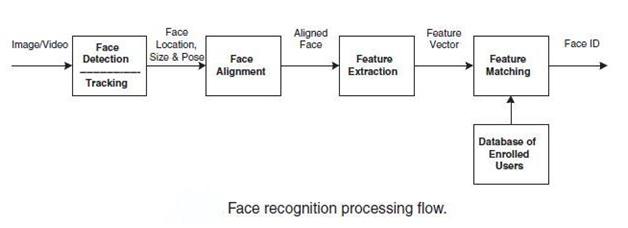
\includegraphics[width=\linewidth]{Bilder/FaceRecognition.png}
\caption{ Phasen der Gesichtserkennung \newline Quelle: https://alitarhini.files.wordpress.com/2010/12/untitled1.png }
\label{fig:Face Recognition}
\end{figure}
Die Detection Phase ist dafür verantwortlich um zu erkennen ob Gesichter vorhanden sind in einem Bild, oder aber Video.
\footcite[Vgl. ][2]{HandbookFaceRec}
In der darauffolgenden Alignment Phase hingegen wird die Lokalisierung der Gesichter genauer, indem Gesichtskomponenten wie Augen, Augenbrauen, oder die Nase genauer lokalisiert werden. Dabei
wird das Bild oder Video ebenfalls normalisiert, indem z.B. die Bildbeleuchtung angepasst wird.
 \footcite[Vgl. ][2]{HandbookFaceRec}
In der Feature extraction hingegen werden die verschiedenen Gesichtskomponenten wie Augen, Nase, Mund, dem Bild oder Video entnommen. Dies ist ein wichtiger Schritt für weitere Prozesse wie
Eye Tracking oder Face Tracking. Alternativ kann sogar eine bestimmte Person anhand der extrahierten Merkmale erkannt werden.
\footcite[Vgl. ][Abstract]{IEEE}
In der letzten Phase, dem Matching, geht es darum die gewonnen Daten mit den in der Datenbank vorhandenen Gesichtern abzugleichen. Wenn eine genügende Übereinstimmung gefunden wurde, wird ein
Match mit einer Person ausgegeben.
  \footcite[Vgl. ][3]{HandbookFaceRec}
Die Anwendungsgebiete von Software die Gesichtserkennung ermöglicht ist mannigfaltig. Sie reicht von Applikationen die ein Gerät wie ein Smartphone entsperren, wenn das Gesicht des Besitzers als
Match ausgegeben wurde, bis hin zur Anwendung in Verbrechensbekämpfung. In jedem dieser Szenarien wird dabei der oben beschriebene Ablauf durchgegangen, und abhängig vom zu liefernden Ergebnis
eine Abschlussaktion vorgenommen.


\subsection{Emotionserkennung}

In diesem Unterkapitel nun sollen Emotionen an sich thematisiert werden, da diese maßgeblich sind für das zu entwickelnde Tool. Eine Definition von Emotionserkennung ist per se nicht schwer zu geben. Prinzipiell beschäftigt sich Emotionserkennung mit der Analyse von Gesichtern und den Emotionen die diese Gesichter darstellen. Jedoch ist der Begriff der Emotionen nicht ganz so einfach zu definieren, wie im folgenden erläutert wird: 

%\begin{itemize}
%\item was ist Emotionserkennu
%\item usecase für emotion recognition
%\item Aiusblick und Kontroverse
%\end{itemize}


\subsubsection{Emotionen}

\begin{itemize}
\item Def. von Emotionen
\end{itemize}
 Grundsätzlich gibt es  verschieden Ansätze Emotionen zu
definieren und einzuteilen. Eine Variante ist dabei die eingangs erwähnte, nicht ganz unumstrittene Einteilung in Basisemotionen. Eine gängige Einteilung ist dabei die verschiedenen
Emotionen in acht Bereiche einzuteilen. Diese Einteilung wurden 1984 von Plutchik postuliert und beinhaltet die Emotionskategorien Angst, Wut, Freude, Trauer, Akzeptanz, Ekel, Erwartung und
Überraschung.
\footcite[Vgl. ][3]{FaceRec}
Jedoch ist dies nicht die einzige mögliche Einteilung. Als weiteres Beispiel teilte MacLean die Emotionen in lediglich sechs Kategorien ein, welche da wären: Verlangen, Wut, Angst,
Niedergeschlagenheit, Freude und Zuneigung.
\footcite[Vgl. ][3]{FaceRec}
Wie sich bereits an den beiden Beispielen zeigt, geht die Meinungen der Forscher dabei  stark auseinander, welche und wie viele Emotionen zu den sogenannten ''Basis Emotionen'' gehören. In
dieser Arbeit werden die Emotionen in sechs Kategorien eingeteilt, in Wut, Trauer, Freude, Ekel, Überraschung und Neutral. Diese Einteilung entspricht an sich keiner gängigen Einteilung, jedoch
wurde diese aus den folgenden Gründen gewählt: \newline
Die hier genannten Emotionen lassen sich gut anhand von Bildern erlernen, da diese zum Teil komplementär und somit eindeutig sind. Es ist aber auch einfacher Testdatensätze zu bekommen für ein
freudiges Gesicht, oder ein überraschtes, als ein Gesicht mit dem emotionalen Ausdruck Akzeptanz. Des Weiteren wurde der Ausdruck ''Neutral'' hinzugefügt. Neutral repräsentiert ein emotionsloses
Gesicht, und somit nach Definition einem Pokerface. Zudem sind die gewählten Emotionen häufig bei dem Test Usecase dieser Arbeit anzutreffen, dem Texas Holdem Poker.


\subsubsection{Abgrenzung zur Gesichtserkennung}
Der grundlegende Unterschied zwischen Emotions- und Gesichtsereknnung liegt nun darin, dass bei der Emotionserkennung selber nicht die agierende Person im Vordergrund steht, sondern die Aktion die sie ausführt.
Bei der Gesichtserkennung hingegen spielt lediglich die Rolle wer eine Aktion ausführt, und ob es einen Treffer in der Datenbank gibt, oder nicht. Wegen dieser Unterschiede ist auch die technische Realisierung eines Prototypen, vor allem im Bezug auf die Architektur,  durchaus unterschiedlich. Dies ist jedoch ebenso von den unterschiedlichen Anwendungszenarien der beiden Verfahren bedingt.
 Denn diese sind ebenso verschieden. Während Gesichtserkennung eher in den Bereich IT-Security oder aber Social Media (Snapchat Filter) eingesetzt wird, ist Emotionserkennung eher Informationsgenerierend.
Zum Beispiel kann durch Emotionserkennung Informationen zugänglich werden wie das Befinden eines Individuums ist, ob emotional betroffen ist, oder aber nicht emotional betroffen wirken möchte und ein Pokerface aufsetzt.
Wegen dieser signifikanten Unterschiede kann daher trotz der Gemeinsamkeiten nicht gesagt werden, dass Emotionserkennung eine Unterkategorie von Gesichtserkennung ist.

\section{Emotionserkennung mithilfe von Deep Learning}

In dem nun folgenden Kapitel wird erörtert wie das Ziel des Prototypen dieser Arbeit - das Erkennen eines Pokerfaces - mittels eines neuronalen Netzes umgesetzte werden kann. Dabei wird weniger auf die generellen Eigenschaften von Neuronalen Netzen Bezug genommen, als auf die in dieser Arbeit spezifischen Aspekte. Diese sind vor allem verschieden Ansätze und Möglichkeiten mittels Machine Learning eine Emotionserkennungssoftware zu erstellen.
\subsection{Dlib vs. Keras}
Libraries werden hier expliziert
\subsection{Supervised vs. Unsupervised Learning}
Layer, Neuronen und Algorithmen explizieren 



\let\cleardoublepage\relax






\chapter{Ergebnis}

In diesem Kapitel wird das Konzept bezüglich der Architektur sowie verwendeter Komponenten und deren Kommunikation dargestellt. Außerdem werden die Aufgrund des erstellten Konzeptes entwickelten Lösungsansätze und Lösungen erläutert. Darin inbegriffen ist vor allem auch das trainierte Modell zum klassifizieren von den vordefinierten Emotionen und das Verifizieren und Testen dieses Modells.

\section{Konzept}

Nachfolgend wird das in der Planungsphase entwickelte Konzept zur Emotionserkennung unter verschiedenen Aspekten erläutert.

\subsection{Architektur}

\subsubsection{Hardware}

Der Einfachheit halber wird als grundlegende Komponente ein handelsüblicher Laptop zum Entwickeln genutzt.  Außerdem wird dabei auf das OpenSource Betriebssystem Ubuntu 18.04.4 LTS in der 64-bit Variante zurückgegriffen. Als zugrunde liegende Ressourcen stehen ein 8 GigaByte Arbeitsspeicher sowie ein Intel Core i5-4210 Quadcore Prozessor mit einer Taktfrequenz von 4 x 2,60 GHz zur Verfügung. Des Weiteren kann die dedizierte Grafikkarte GeForce 820M mit einem Grafikkartenspeicher von 2046 MB verwendet werden. Der Festplattenspeicher von 500 GB kann im Umfang dieser Arbeit vernachlässigt werden, da es im Zusammenhang mit Gesichts- bzw. Emotionserkennung primär darauf ankommt, wie viel Rechenleistung zur Verfügung steht und nicht wie groß die Speicherkapazität des Laufwerks ist. Um das rechenintensive Trainieren des Modells zur Emotionserkennung in akzeptabler Zeit zu garantieren, soll die Rechenleistung des Prozessors und der Grafikkarte vollständig genutzt werden können.

\subsubsection{Programmierumgebung}

Aufgrund der Vorkenntnisse und Relevanz innerhalb des Studiums soll die Programmiersprache Python in aktuellster Version (3.6.9) vorrangig verwendet werden, jedoch kann unter gegeben Umständen auch die Programmiersprache C++ eingesetzt werden, was noch zu prüfen ist. Auf eine bestimmte IDE wie PyCharm, Emacs oder Visual Studio Code wird sich an dieser Stelle nicht festgelegt, da dies jedem Entwickler selbst zu überlassen ist. Diesbezüglich sind nur Einschränkungen aufgrund der gewählten Rechnerarchitektur und der Programmiersprache zu berücksichtigen. \newline
Zur Entwicklung einer Emotionserkennung sollen als grundlegende Komponenten die Programmbibliothek für Bildverarbeitung OpenCV und das Framework Tensorflow bzw. die Deep-Learning-Bibliothek Keras verwendet werden. Da das Einsatzgebiet von OpenCV in der Bildverarbeitung liegt, soll die Bibliothek dazu genutzt werden, den Input so zu verändern, dass dieser vom Modell zum trainieren oder vorhersagen einer oder mehrerer Emotionen verwendet werden kann. Für den wesentlichen Teil der Arbeit, das Entwickeln eines Modells, welches menschliche Emotion anhand eines Bildausschnittes von einem Gesichts erkennen kann, ist die Deep-Learning-Bibliothek Keras zu verwenden.

\subsection{Interaktionskonzept}

Von der Metaebene aus betrachten, steht noch die Planung eines Interaktionskonzeptes aus, welche nun genauer erläutert wird. Die Bildbverarbeitungsbibliothek OpenCV soll dazu verwendet werden, eine grafische Benutzeroberfläche (GUI) in Form eines Fensters zu entwickeln, mit dessen Hilfe dem Nutzer die Möglichkeit geboten wird, entweder Aufnahmen durch die integrierte Webcam selber als Input zu liefern oder dafür ein von ihm gewähltes schon bestehendes Bild auszuwählen. Das vom Nutzer gelieferte Bild soll entsprechend bearbeitet werden, um anschließend eine Emotion zu erkennen und den entstandenen Output an eine durch OpenCV generierte Oberfläche weiterzugeben. In welcher Form der Output dem Nutzer letztendlich dargestellt wird, als Grafik, einfache Textausgabe oder audiovisuell ist noch zu entscheiden.\newline
Zusammenfassend kann man also sagen, dass der Nutzer aufgrund der Übersichtlichkeit und der Einfachheit halber lediglich mit den von OpenCV generierten Oberflächen interagiert und sich zu keinem Zeitpunkt mit der dahinterliegenden Komponente Keras befassen muss.\newline
Es wird sich auch die Option vorbehalten, den Input webbasiert zu liefern und dem Nutzer auch auf gleiche Art und Weise den Output zurückzuliefern. Um die Komplexität des Projektes weiterhin auf die wesentlichen Bestandteile der Emotionserkennung zu beschränken und nicht unnötig zu erhöhen, wird diese Möglichkeit jedoch vorerst nicht weiter berücksichtigt.

\section{Umsetzung der Lösung}

Während der weiteren Ausarbeitung des Konzeptes und der darauf basierenden Umsetzung sind letztendlich zwei verschiedene Lösungen entstanden. Aufgrund von Problemen die innerhalb des Entwicklungsprozesses im Zusammenhang mit dem Hardwarekonzept aufgetreten sind, konnte das Projekt so wie es geplant war nicht zu Ende gebracht werden. Da diese Lösung jedoch als Grundlage für die letztendlich finale Lösung diente, werden nachfolgend beide Umsetzungen genauer erläutert.

\subsection{Stand-Alone Lösung mit Schwerpunkt OpenCV}

In diesem Kapitel wird die Umsetzung der auf dem entwickelten Konzept basierenden Lösung näher erläutert. Es handelt sich dabei um den Stand-Alone Laptop mit installiertem Ubuntu 18.04.4 LTS wobei der Input und Output auf OpenCV GUIs basiert.

\subsubsection{Input GUI}

\subsubsection{Dataset}

\subsubsection{Training}

\subsubsection{Verzeichnisstruktur}
 	
\subsection{Webbasierte Lösung}

\subsubsection{Dataset}

\subsubsection{Modell}

Nachfolgend wird das für die Emotionserkennung erstellte Modell mit den jeweils einzelnen Layern näher erläutert und \ref{fig:Model Summary}
\begin{figure}[h]
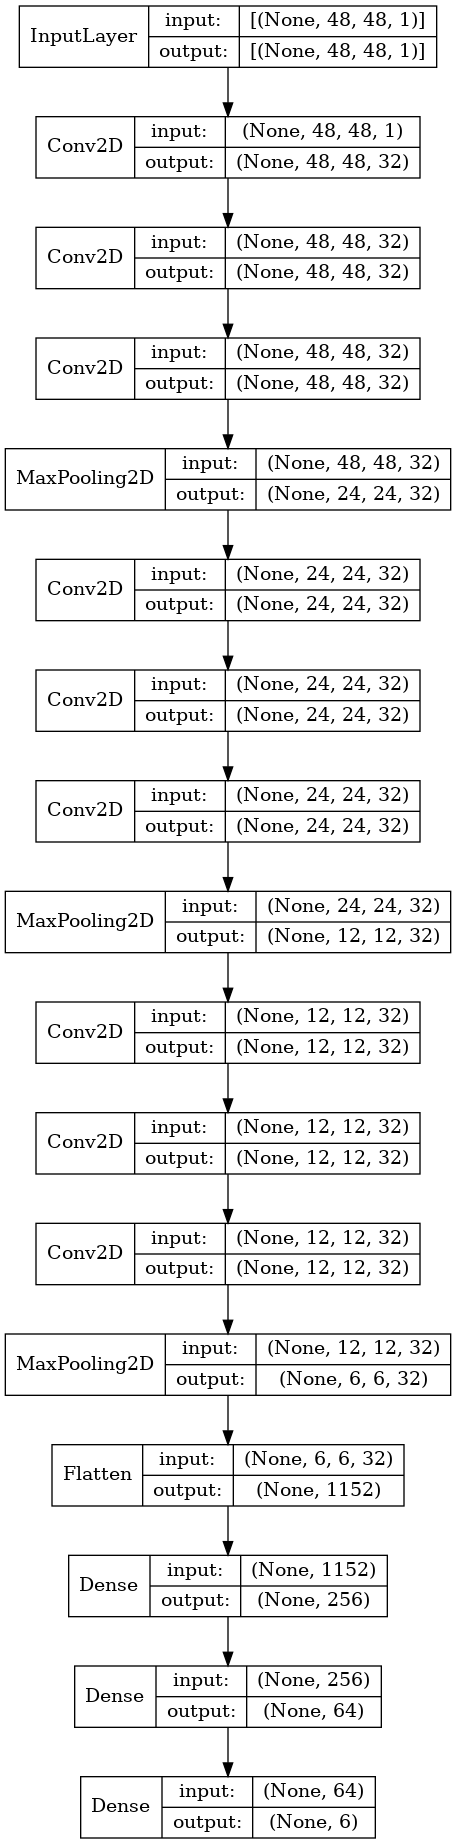
\includegraphics[viewport=0 1177 300 1844]{Bilder/ModelSummary.png}
\end{figure}
\begin{figure}[h]
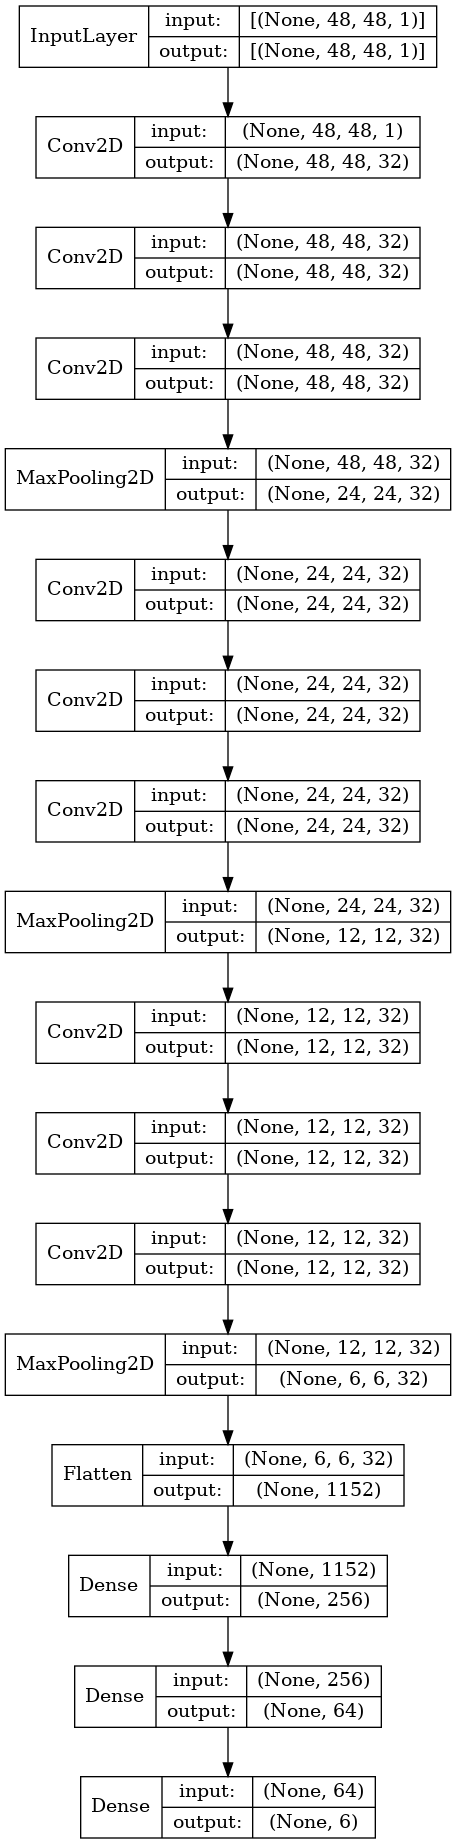
\includegraphics[viewport=-14 150 300 1030]{Bilder/ModelSummary.png}
\end{figure}
\begin{figure}[h]
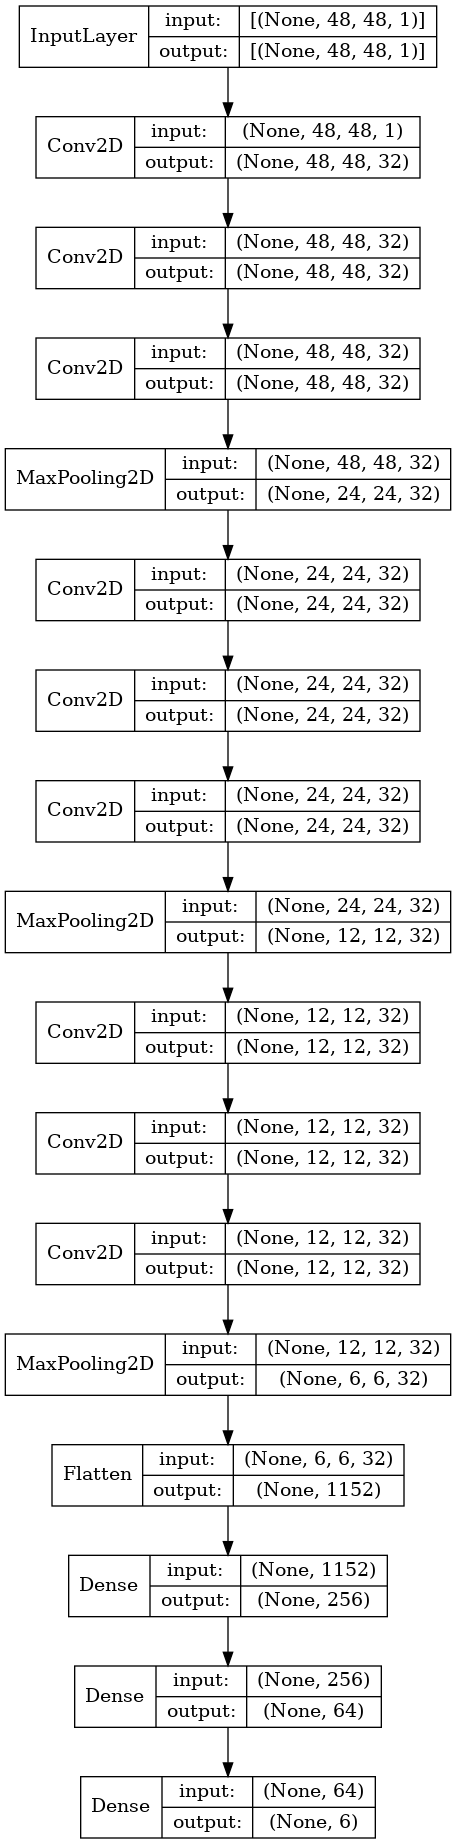
\includegraphics[viewport=0 0 455 510]{Bilder/ModelSummary.png}
\caption{ Model Summary with several Layers and I/O Shapes }
\label{fig:Model Summary}
\end{figure}

\subsubsection{Trainieren des Modells}

\subsubsection{Testen des Modells}

\subsubsection{Webserver}

\subsubsection{Jupyter Notebook}

\subsubsection{Verzeichnisstruktur}

\let\cleardoublepage\relax





\chapter{Diskussion}


Das nunmehr letzte Kapitel soll sich mit der kurzen Zusammenfassung der Ergebnisse des letztens Teils und deren Bewertung widmen. 
%Die Ergebnisse aus dem letzten Kapitel noch einmal zusammenfassen?
Des Weiteren sollen die angewandten Methoden reflektiert werden,
offene Fragen beantwortet und auch weitere Punkte aufgezeigt werden die verbessert oder noch implementiert werden können. Dazu soll zunächst die Ergebnisse kurz zusammengefasst werden.


\section{Reflexion der Ergebnisse}

\subsection{Alternativen}


\section{Reflexion Vorgehen}

Mehr darauf eingehen dass das Kontrovers ist und auch die Basisemotionen kontrovers sind --  aber keine andere Möglichkeit vorhanden 



\section{Reflexion der Literatur}

Bezüglich der Literatur ergeben sich nun einige Schwierigkeiten. Dies liegt unter anderem daran, dass das generelle Thema der Gesichts und Emotionserkennung immer noch vor allem aus
psychologischer Sicht in der Literatur behandelt wurde. Zwar gibt es Fachbücher auch aus informationstechnischer Sicht, welche ebenfalls in dieser Arbeit verwendet wurden.



\section{Offene Implikationen}





\chapter{Ausblick}


\section{Alternative Ansätze zur Umsetzung von Emotionserkennung}

In diesem Abschnitt nun werden verschiedene alternative Ansätze dargestellt und expliziert, die dazu verwendet werden können um Emotionen zu erkennen.
Dieses Unterkapitel beschäftigt sich mit alternativen Ansätzen zu den bereits explizierten Basisemotionen. Diese sind wie bereits erwähnt umstritten, was die Frage zulässt warum diese überhaupt
verwendet werden sollten. Ein weiterer kreativer Ansatz zur Erkennung von Emotionen wäre die Analyse der Stimmlage.
Dieser Ansatz beruft sich darauf, dass das Sprachzentrum eines Menschen einer der wichtigsten Aspekte der Kommunikation und somit auch der Preisgabe von Informationen über den emotionalen Zustand eines Individuums ist.
\footcite[Vgl. ][Abstract]{EmotionInSpeech}
Dieser Ansatz ist jedoch nicht zielführend, da hier hauptsächlich die Stimme analysiert wird. Von einer Stimme kann nun auf eine Emotion geschlossen werden. Für den Usecase ist dieser Ansatz allerdings ungeeignet, aus folgenden Gründen:
\newline
Es kann möglich sein eine Emotion anhand der Sprache zu erkennen. Das Äquivalent eines Pokerfaces wäre dementsprechend eine neutrale Stimmlage, welche keine Emotionen suggeriert. Nun kann aber keine Aussage getroffen werden aus welchen Gründen eine Person neutral spricht. Es könnte von einem Pokerface stammen, oder einer monotonen Sprechweise, oder einen gelangweilten Gemütszustand. Dies ist nicht eindeutig identifizierbar. Gleiches könnte nicht über ein neutrales Gesicht gesagt werden, da dies gemeinhin als Pokerface bezeichnet wird. %Spricht das nicht auch gegen unser Vorgehen?
Ein weitere Ansatz wäre die Analyse der derzeit vernommenen Musik. Diese kann einem bestimmten Gemütszustand zugesprochen werden, welches auf eine aktuelle Emotion übertragbar ist.
\footcite[Vgl.][1]{MusicEmotion}
Ziel dieses Forschungszweiges ist es daher die hinter Liedern oder Klängen stehenden Emotionen zu ermitteln und diese entsprechend zu kategorisieren.
Dieser Ansatz erscheint zunächst durchaus interessant, hat jedoch genauso Nachteile wie die Analyse von Emotionen anhand von Bildern die Basisemotionen zeigen. %Spricht wieder gegen unser Vorgehen
Dieser liegt hier unter anderem in der Genauigkeit der Analysen. So z.B. lieferte ein Testprojekt an der Russischen HSE (Higher School of Economics) das Ergebnis von einer maximalen Genauigkeit von 71\%.
\footcite[Vgl. ][Abstract]{EmotionInSound}
In dem Versuchsaufbau wurden Spektrogramme von Klangfragmenten ausgewertet und versucht mittels Neuronalen Netzen eine Klassifikation der hinter dem Klang liegenden Emotion zu erreichen.
\footcite[Vgl. ][Abstract]{EmotionInSound}
Der generelle Ansatz anhand von Musik die Emotion eines Individuums abzulesen ist zwar praktikabel und von dem Versuchsaufbau auch vergleichbar zu dem Ansatz bereits gelabelte Bilder zu verwenden. Jedoch lässt sich auf diese Weise aus zwei Gründen nicht die eigentliche Zielaufgabenstellung ableiten, das Erkennen eines Pokerfaces. Zum einen handelt es sich in dieser Arbeit um eine visuelle Problemstellung, in welcher das Erkennen des Gemütszustandes anhand des Gesichtsausdruckes erkannt werden soll, also einem vorhandenen bzw. nicht vorhandenen Pokerface. Zum anderen würde die Analyse von Musik einen Rückschluss auf den allgemeinen Gemütszustand des Betroffenen folgern und nicht eine kurzzeitige Stimmungsschwankung aufgrund beispielsweise eines schlechten Blattes, wie in diesem Usecase.


\let\cleardoublepage\relax
\newpage

\printbibheading
\printbibliography[type=book,heading=subbibliography,title={Literaturquellen}]
\pagestyle{empty}
\printbibliography[type=misc,heading=subbibliography,title={Sonstige Quellen}]
\pagestyle{empty}
\newpage
\pagestyle{empty}

\end{document}
